\chapter{関連研究}
\thispagestyle{fancy} %ヘッダー・フッターの設定

%% 「。」を「.」にしたり、「、」を「,」にしたりするのは後で置換で一括でやります。

画像のレジストレーション手法は主に2つのモダリティ間の画像の類似度評価の技術と画像を変形させる技術に基づいて構成されている.
ここでは類似度評価手法および変換手法について主に使われている手法を述べてから, 具体的なレジストレーション手法について確認する.
また, 具体的な手法については特に医療画像に使用される技術について言及する.

\section{マルチモーダルレジストレーション}

%% 「。」を「.」にしたり、「、」を「,」にしたりするのは後で置換で一括でやります。

医療画像レジストレーションの中でも、モダリティを超えて画像の整合性を考慮するマルチモーダルレジストレーションは非常に難易度が高く、盛んに研究が行われているにも関わらず、未だに精度の高いレジストレーションは実現していない。
画像レジストレーションの精度は深層学習を用いることによって精度および速度が飛躍的に向上したものの、マルチモーダルレジストレーションに関しては

\subsection{古典的手法}

\subsection{類似度を用いた手法}

\subsection{強化学習を用いた手法}

\subsection{教師あり学習を用いた手法}

\subsection{半教師あり学習を用いた手法}

\subsection{教師なし学習を用いた手法}
 
\section{転移学習}
% DONE

%% 「。」を「.」にしたり、「、」を「,」にしたりするのは後で置換で一括でやります。

転移学習やドメイン適応は、あるタスクで学習したことを別のタスクの汎化能力向上に役立てようとする状況を指す言葉である。
マルチタスク学習との決定的な差は、マルチタスク学習がソースタスクとターゲットタスクを同時に学習するのに対して、転移学習はターゲットタスクを最も重要視する点にある。
深層学習を用いた医療画像処理において、学習データの欠如は非常に重要な問題であり、転移学習やドメイン適応を利用した少数データで十分に汎化したモデルを得る研究が非常に重要な課題になっている。    
前節までにおいて紹介してきた機械学習モデルの前提として、訓練データとテストデータは同様の分布であるという暗黙の了解がある。
例えば、カメラで撮影したRGB画像を入力として想定した、犬種判別モデルに赤外画像を入力しても良い精度は得られない。
また、上記のモデルに同じRGB画像を入力したとしても、猫の画像を入力しても無意味な結果が得られるだけである。
このように、多くの機械学習モデルは非常に厳しい前提条件の元にうまく機能するが、大抵の場合にはこの前提条件は適用されない。
しかし、仮に犬種判別のモデルの知識が猫種判別の知識に利用できる場合、犬種判別モデル作成に利用していたデータよりも少数のデータで猫種判別モデルを作成することが可能になる可能性がある。

このように、多量のラベリング作業によるコストおよび労力緩和のために、転移学習は非常に良い選択肢となりうる。
深層学習モデルの転移学習では、一般にImageNet用に設計された標準的なモデルが使用される。
これは特に視覚的なカテゴリ(画像に関するタスク)に限定されるが、視覚的なカテゴリではエッジや形などの概念、幾何学的変化による影響や、証明の変化などの特徴が共通であり、ImageNetで訓練されたモデルこれらを抽出可能なパラメータはすでに所持していると言える。
故に、出力に近い部分を学習することにより、様々なタスクへの応用が可能となる。

医療画像ではImageNetで訓練されたモデルに対して医療用画像で微調整を行い、胸部X線画像の解釈\cite{majkowska2020chest}、アルツハイマー病の早期発見\cite{ding2019deep}、目の疾患の特定\cite{varadarajan2018deep}などに使用している例がある。

\subsection{転移学習の定義}
    転移学習は様々な文献で多様な定義が行われている\cite{pan2009survey, zhu2011heterogeneous, shao2014transfer, zhang2017transfer}。
    転移学習やドメイン適用に関する概念は比較的新しく、まだ決まっていないことに加えて、本論文で扱うドメイン適応の説明のためには詳細な分類は不要であることから、ドメイン適用の位置づけを理解するために最低限必要である、最も基本的な分類\cite{pan2009survey}に関して述べる。
    
    まず、最も基本的な定義を理解するためには「ドメイン」および「タスク」の概念を定義する必要がある。
    ドメインとは、データ空間のことであり、ある特定の確率分布$P(X)$に従って分布しているデータ$X=\{x_1,x_2,...,x_n\}\in X$で張られる特徴量空間Xのことを指す。
    そして、タスクとはあるドメイン$D=\{X,P(X)\}$が与えられた際のラベル$Y=\{y_1,y_2,...,y_n\}\in Y$および、Xから学習可能な関数$f(\cdot )$から構成され、$T=\{Y,f(\cdot)\}$で表される。
    このとき、$X$および$Y$の要素は互いに対応している。
    
    そして、転移学習を考える際に最も重要なものが、ドメインの差異である。
    元となる知識があるドメインのことをソースドメインとして$D_S$と表し、転移先であるドメインをターゲットドメインとして$D_T$として表す。
    
    この条件の元での転移学習の定義は以下のようになる\cite{pan2009survey}。
    \begin{quote}
        ソースドメイン$D_S$と学習タスク$T_S$、ターゲットドメイン$D_T$と学習タスク$T_T$が与えられた場合、転移学習は$D_S \neq D_T$または$T_S \neq T_T$である$D_S$および$T_S$の知識を用いて、$D_T$における予測関数$f_T(\cdot)$の学習を改善することを目的としたもの。
    \end{quote}

\subsection{転移学習の分類}
    前項で示した転移学習の定義では、転移学習は$D_S \neq D_T$または$T_S \neq T_T$である場合を想定しているため、転移学習は様々なケースに分類することが可能である。
    転移学習の様々なケースは、データの特性に注目することで1)帰納的転移学習、2)伝達転移学習、3)教師なし転移学習の3種類に分類することが可能である。
    \begin{enumerate}
        \item 帰納的転移学習(Inductive Transfer Learning)\\
            帰納的転移学習は、転移学習の中でも特に$T_S \neq T_T$であるものを指す。この枠組みで更に特徴的なのは$T_S$および$T_T$がどちらも利用可能であることである。
            さらに、これらの中でも$D_S$かつが$D_T$のデータが豊富である場合、マルチタスク学習と呼ばれ、$D_T$のみデータが豊富である場合には半教師あり学習(自己教師あり学習, self-supervised learning)と呼ばれる。
        \item 伝達転移学習(Transductive Transfer Learning)\\
            伝達転移学習は、転移学習の中でも特に$D_S \neq D_T$であるものを指す。この学習ではソースドメインに多くのラベルが存在する一方、ターゲットドメインに十分な数のラベルが存在しない。
        \item 教師なし転移学習(Unsupervised Transfer Learning)\\
            教師なし転移学習は、帰納的転移学習と同様に$T_S \neq T_T$である場合を想定しているが、それぞれのタスクが独立せずに関連しているケースで用いる。
            この枠組みで更に特徴的なのはソースドメインおよびターゲットドメインのどちらでも十分なラベルデータが存在しないことである。
            故に、教師なし転移学習では次元削減やクラスタリングによって学習タスクを解くことが求められる。
    \end{enumerate}
    上記の転移学習の設定及び関連領域に関する分類を以下の表\ref{ClassificationOfTL}にまとめた

    \begin{table}[ht]
    \caption{Classification of Transfer Learning Settings and Related Domains\cite{pan2009survey}.}
    \resizebox{\textwidth}{!}{%
    \begin{tabular}{|l|l|l|l|}
    \hline
    Transfer Learning Settings                   & Related Areas            & Source Domain Label & Target Domain Label \\ \hline
    \multirow{2}{*}{Inductive Transfer Learning} & Multi-task Learning      & Available           & Available           \\ \cline{2-4} 
                                                 & Self-supervised Learning & Unavailable         & Available           \\ \hline
    Transductive Transfer Learning & \begin{tabular}[c]{@{}l@{}}Domain Adaptation, Sample \\ Selection Bias, Co-variate Shift\end{tabular} & Available & Unavailable \\ \hline
    Unsupervised Transfer Learning               &                          & Unavailable         & Unavailable         \\ \hline
    \end{tabular}%
    }
    \label{ClassificationOfTL}
    \end{table}

\subsection{転移学習のアプローチ}
    転移学習にはモデルの知識を転移させるために様々なアプローチが存在する。
    このアプローチ方法は、転移対象によって分類が可能である。
    以下では、転移学習を転移対象とその手法に基づいて転移学習を4つに分類する。
    \begin{enumerate}
        \item Instance-Transfer\\
            Instance-Transferの関心領域はデータ自体であり、ソースドメインのデータをターゲットドメインで利用するために、ソースドメインのデータを重み付けする手法である。
        \item Feature-representation-transfer\\
            Feature-representation-transferの関心領域はモデルのパラメータであり、ソースおよびターゲットのドメイン自体の差や、それぞれのドメインでの分類誤差を最小化する特徴量を見つける、または学習する手法である。
        \item Parameter-transfer\\
            Parameter-transferの関心領域はモデルのパラメータであり、ソースドメインで作成したモデルおよびターゲットモデルで作成したモデルにおける、パラメータの共通点を発見することによって、どちらのドメインでも用いることの可能なパラメータを作成するような手法である。
        \item Relational-knowledge-transfer\\
            Relational-knowledge-transferの関心領域は抽出後の特徴量であり、同一のモデルによって抽出されたそれぞれのドメインでの特徴量の対応付けを行い、知識のマッピングを行う手法である。
    \end{enumerate}

\subsection{医療画像応用における問題点}
    前項で触れたように転移学習は深層学習の医療画像応用において広範に利用されている。
    しかし、転移学習の正確な効果はまだ十分に理解されていない。
    医療画像だけでなく、特定のタスクに限定的に用いられるモデルに対して、ImageNetで訓練されたモデルの重みを転移学習に用いるのは意味がない場合が多い。
    特に医療画像では、ImageNetでは画像の主題を問われているのに対し、画像の特定の部分のみが関心対象であったり、データセットの規模や画像のスケールの隔たりなど、様々な差異が存在する。
    そのため、医療画像では転移学習によりパフォーマンスが大幅に向上することはなく、事前学習を適用しなかった単純なモデルも同等の精度を発揮することが示されているケースも報告されている\cite{raghu2019transfusion}。

\section{ドメイン適応}
% TODO
% ドメイン適応のアプローチ
% 医療画像におけるドメイン適応
% 本論文におけるドメイン適応(提案手法の方に回す?)

%% 「。」を「.」にしたり、「、」を「,」にしたりするのは後で置換で一括でやります。

ドメイン適応は、大量のラベルデータの不足に対処するための新たな学習手法であり、転移学習の特殊なケースとして位置づけられる。
前節の定義に従うと、ドメイン適応は転移学習の中でも特に$D_S \neq D_T$であるものを指す。

本節では、Wanら\cite{wang2018deep}の論文による分類を元に、特に深層学習に注目して、ドメイン適応の定義と分類を示した後に、医療画像レジストレーションタスクがドメイン適応においてどのように分類されるのかを示す。

\subsection{ドメイン適応の分類}
    深層学習のような手法を用いない場合、ドメイン適応のアルゴリズムは2つに大別できる。
    1つ目は、ソースドメインでのラベルをターゲットドメインで利用するために、ソースドメインのデータ自体に重み付けをするような転移学習(Instance Transfer)である。
    2つ目は、ソースドメインおよびターゲットドメインの差や、モデル誤差を軽減する特徴量を見つけるような転移学習(Feature representation transfer)である。

    深層学習におけるドメイン適応を考慮する際に、このドメインの違いについての形態は、 それぞれのドメインが同質であるかどうかによってさらに2つに分類することが可能である。
    先述したように、ドメイン適応は転移学習の特殊なケースとして位置づけられ、$D_S \neq D_T$の場合を想定している。
    しかし、この定義ではこの差異がデータの分布によるものなのか、特徴空間の差異のことなのかは明確にされていない。
    そこで、、Wanら\cite{wang2018deep}はデータ分布のみが異なり、特徴空間は同一である場合をHomogeneous DA、特徴空間自体が異なる場合をHeterogeneous DAとして分類している。
    
    Heterogeneous DAは特徴空間自体が異なる場合であるが、取り扱うメディア自体が同じ場合と異なる場合でさらに2種類に分けることができる。
    取り扱うメディア自体が同じ(例:画像対画像)場合は、例えばデータ取得に利用したデバイスの差(可視光、近赤外、奥行き付映像など)や、画像スタイルの差異(絵と写真など)などのケースが考えられ、取り扱うメディア自体が異なる場合(例:画像対言語)には、メディアが同じ場合よりもドメインの差異が非常に大きくなる。

    深層学習モデルにおけるドメイン適応を考慮する際には、基本的にInstance Transferのような手法について議論されることは少ない。
    深層学習モデルをどのように設計すれば異なるドメインの表現を獲得することが可能かを議論することが大半であり、本論文ではこのような汎用的な特徴表現を学習することを前提としてドメイン適応を分類する。
    具体的には、データの種類によって学習の方法は「教師あり学習」「半教師あり学習」「教師なし学習」の3つに大別することができる。
    つまり、深層学習のOne-Stepドメイン適応は、ドメインの質に関して2通り、学習方法に関して3通りの分岐が存在し、合計で6つに分類することが可能であることが分かる(図\ref{category_of_DA})。
    
    \begin{figure}[ht]
      \centering
      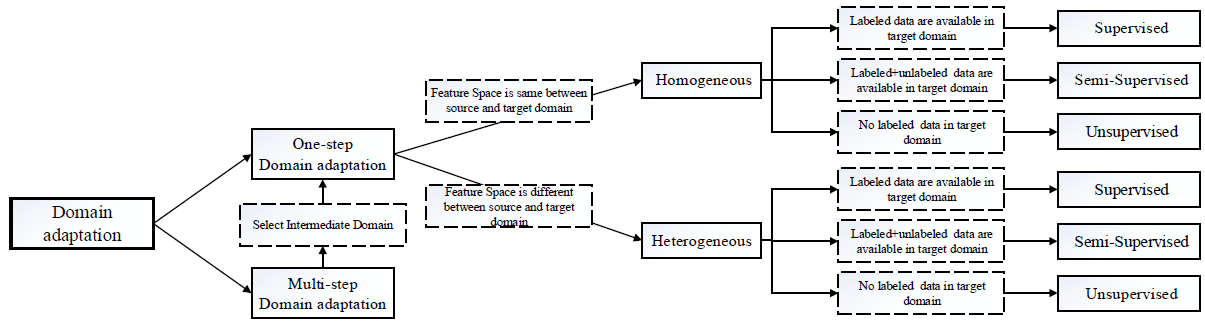
\includegraphics[width=\linewidth]{2_related_works/img/category_of_DA.png}
      \caption{An overview of different settings of domain adaptation\cite{wang2018deep}.}
      \label{category_of_DA}
    \end{figure}

    また、ドメインの特性が互いにあまりにも違う場合には、稀に中間のドメインを経由してドメイン適応を行う例(Multi-Step Domain Adaptation)も存在するが、本論文ではそのような例は扱わない。
    

\subsection{ドメイン適応のアプローチ}
    深層学習モデルをドメイン適応させるために、様々なアプローチが考案されている。
    これらのアプローチは大きく分けて3つに分類することができる\cite{csurka2017domain}。
    \subsubsection{Discrepancy base}
        discrepancyベースのアプローチは、教師データを用いて深層学習モデルを最適化する中でドメインシフトに対応する手法である。
        
        用いる損失関数や何を基準にするかによってさらに細分化されるが、多くが通常の深層学習モデルの訓練と同様に訓練が可能である。
        
        
        
        
    \subsubsection{Adversarial base}
        Adversarialベースのアプローチは、GANを用いてドメインの混合を促す手法である。
    \subsubsection{Reconstruction base}
        Reconstructionベースのアプローチは、補助的なタスクとして画像再構成を課すことにより、特徴量の普遍性を確保することを目指す手法である。
    
\subsection{医療画像におけるドメイン適応}
    医療画像におけるドメイン適応は、


\subsection{本論文におけるドメイン適応}
    本論文では、転移学習の中でも特にドメイン適応に焦点を当てる。
    すなわち、想定するのは$D_S \neq D_T$である状態であり、転移対象に関してはモデルのパラメータを想定する。
    %これはMR-CTなど、画像モダリティの違いを指す。
    基本的に後に述べる敵対的手法\cite{goodfellow2014generative}を用いてモデルを訓練することによりパラメータのドメイン適応を行い、2つのドメインに共通して利用できるモデルを作成することを目標とする。
    つまり、転移学習の枠組みにおいて、本研究はFeature-representation-transferを用いて伝達転移学習を行うことに焦点を当てている。
    しかし、ラベルの有無などの点で細かい定義から多少外れていることに注意されたい。
    次節ではドメイン適応について詳しく述べる。
